\section{Empirical Results and Scaling Laws}
\label{sec:experimental_analysis}

This section presents a comprehensive empirical investigation into the scaling behavior of RL for post-training LLMs. We first examine scaling behaviors under compute and data constraints, then analyze independent scaling dimensions, data reuse strategies, and finally evaluate generalization performance together. To ensure robust conclusions, each configuration is repeated \textbf{three times} for both base and instruct models ranging from 0.5B to 72B.

\subsection{Compute-Optimal Scaling}

\label{subsec:compute_scaling}
To characterize the scaling behavior under computational limits, we first formalize the Compute-Constrained Scenario. Given a fixed computational budget $C$, we seek to identify the optimal model size $N$ (and the corresponding data allocation $D$) that minimizes the final test loss. This can be expressed as the following constrained optimization problem:
\begin{equation}
\label{eq:compute-constrained}
    \underset{N,~D}{\argmin} \ L(N, D) \quad \text{s.t.}\quad \mathrm{FLOPs}(N,D) = C_{\text{const}},
\end{equation}
% \vskip 0.1in

To solve this, we train 0.5B–72B models and measure test loss as a function of cumulative FLOPs $C$. As shown in Figure~\ref{fig:loss_vs_compute_exp}, larger models consistently outperform smaller ones under the same compute budget for both base and instruct variants. \tzl{These plots include both Inter-model Extrapolation (fitted on 0.5B-32B and extrapolated on 72B) and Intra-model Prediction (predicting the remainder of training from initial steps) to demonstrate the predictive power of our derived scaling law.} The loss–compute relationship follows a log-linear trend, which can be modeled by a power-law:
\begin{equation}
\label{eq:compute_law}
\resizebox{\columnwidth}{!}{$
\begin{aligned}
    \log(L(N,C)) = -k_C(N) \cdot \log(C) + E_{C}(N), \\
    \ \text{where} \  k_C(N) = \left(\frac{K_{Cmax}}{1+\frac{N_{C}}{N}}\right)
\end{aligned}
$}
\end{equation}
To validate the predictive capability of Eq.~\ref{eq:compute_law}, we conducted two levels of evaluation under the protocols defined in Section \ref{sec:experimental_setup}. First, applying \textbf{Inter-model Extrapolation}, we fitted the scaling parameters on smaller models (0.5B–32B) to estimate the learning efficiency $k_C(N)$ for the 72B model. As illustrated in Figure \ref{fig:loss_vs_compute_exp_a} and \ref{fig:loss_vs_compute_exp_b}, the predicted efficiency aligns closely with the actual performance of the 72B model. Second, using \textbf{Intra-model Prediction}, we forecasted the remaining loss trajectory of specific models based solely on early training steps (Figure \ref{fig:loss_vs_compute_exp_c} and \ref{fig:loss_vs_compute_exp_d}), confirming the formula's robustness across different training stages.

\tzl{We further analyze learning efficiency term $k_C(N)$ in Eq.~\ref{eq:compute_law}. As Figure \ref{fig:coef_k_c} shows, $k_C(N)$ grows with model size $N$, meaning larger models consistently have higher learning efficiency. However, the efficiency gain from model scale is not uniformly linear. Beyond 32B, the increase in $k_C(N)$ diminishes, leading to efficiency saturation.} 

This saturation is manifested as a distinct performance crossover in Figure~\ref{fig:loss_vs_compute_exp}: In contrast to the immediate dominance of larger models in smaller parameter regimes, the 32B model outperforms the 72B counterpart initially under equivalent compute budgets, as the smaller model size inherently enables more training steps. We believe this observation reveals a latent trade-off between model scale and training steps in compute-constrained scenarios.



\subsection{Data-Optimal Scaling}
\label{subsec:data_scaling}
In many practical applications, the bottleneck lies not in compute but in the availability of high-quality reasoning data. We define the Data-Constrained Scenario as determining the model size $N$ that yields the lowest test loss given a limited amount of unique training data $D$:
\begin{equation}
    \label{eq:data-constraint}
    \underset{N,~C}{\argmin} \; L(N, C) \quad \text{s.t.} \quad D = D_{\text{const}}.
\end{equation}
% ==================================================================
% 第一幅图：Inter-model Prediction (跨模型预测)
% ==================================================================
% ==================================================================
% 第一组图：Inter-model Prediction (跨模型预测)
% ==================================================================
\begin{figure*}[t]
    \centering
    % --- 子图 (a) ---
    \begin{subfigure}[b]{0.48\textwidth}
        \centering
        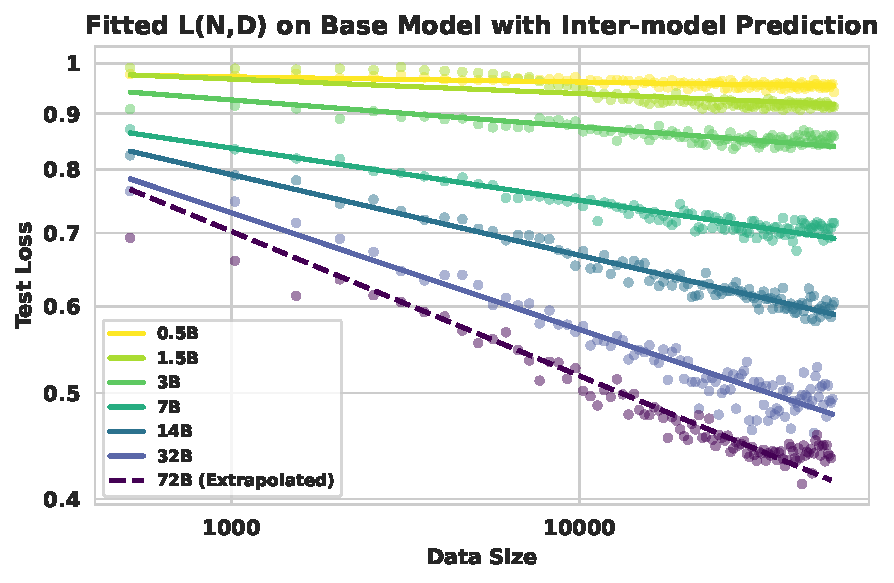
\includegraphics[width=\linewidth]{./figures/outputs/outputs/extrap_base_holdout_N_E_ErrRate.pdf}
        \caption{\tzl{Inter-model Prediction for Base Model}}
        \label{fig:inter_base}
    \end{subfigure}
    \hfill
    % --- 子图 (b) ---
    \begin{subfigure}[b]{0.48\textwidth}
        \centering
        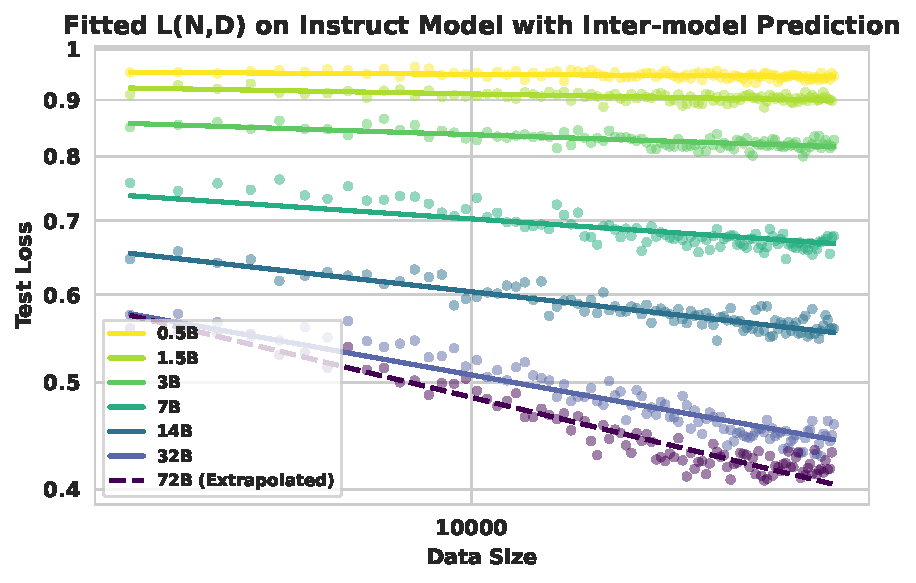
\includegraphics[width=\linewidth]{./figures/outputs/outputs/extrap_instruct_holdout_N_E_ErrRate.pdf}
        \caption{\tzl{Inter-model Prediction for Instruct Model}}
        \label{fig:inter_instruct}
    \end{subfigure}
    
    % --- Caption: 结合了预测方法 + 你指定的完整结论 ---
    \caption{\textbf{Inter-model Prediction in data scenario.} 
    The scaling law parameters are fitted on smaller models (0.5B--32B) to \textbf{predict} the learning efficiency of the largest model (72B, represented by dashed lines). 
    The accurate alignment validates that the superior sample efficiency of larger models follows a predictable trajectory, confirming that performance gains scale consistently up to 72B.}
    \label{fig:loss_vs_data_inter}
\end{figure*}

\begin{figure*}[b]
    \centering
    % --- 子图 (c) ---
    \begin{subfigure}[b]{0.48\textwidth}
        \centering
        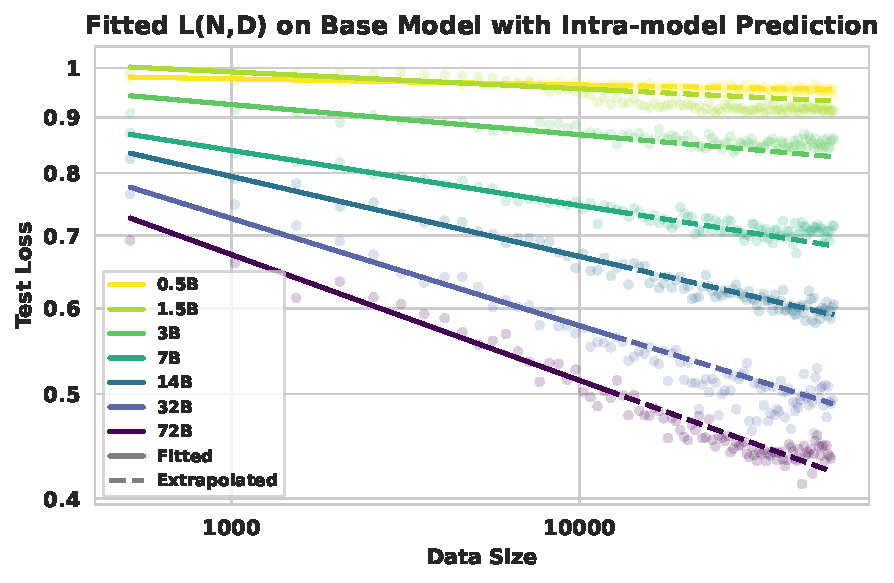
\includegraphics[width=\linewidth]{./figures/outputs/outputs/predict_base25_base_holdout_N_E_ErrRate.pdf}
        \caption{\tzl{Intra-model Prediction for Base Model}}
        \label{fig:intra_base}
    \end{subfigure}
    \hfill
    % --- 子图 (d) ---
    \begin{subfigure}[b]{0.48\textwidth}
        \centering
        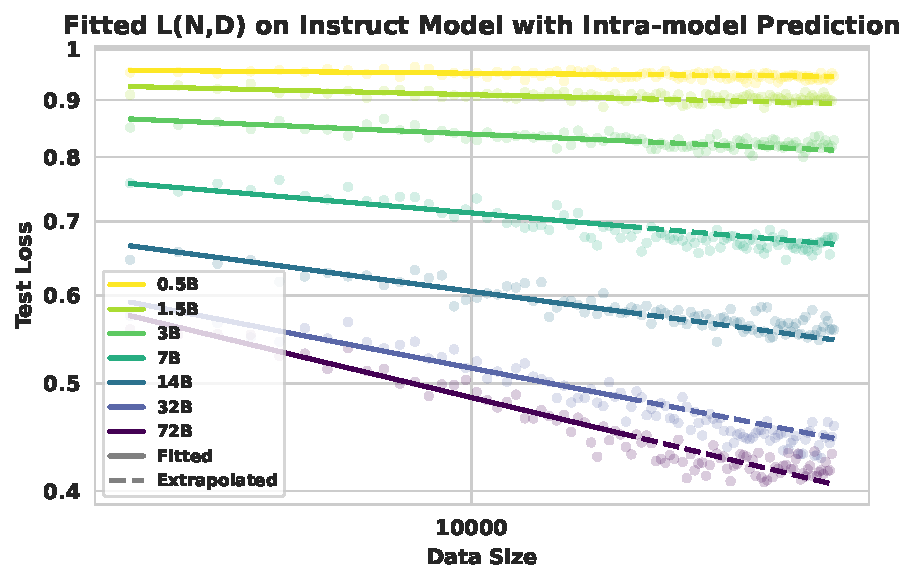
\includegraphics[width=\linewidth]{./figures/outputs/outputs/predict_instruct40_instruct_holdout_N_E_ErrRate.pdf}
        \caption{\tzl{Intra-model Prediction for Instruct Model}}
        \label{fig:intra_instruct}
    \end{subfigure}
    
    % --- Caption: 结合了预测方法 + 结论的可外推性 ---
    \caption{\textbf{Intra-model Prediction in data scenario.} 
    The loss trajectory is fitted using initial training data steps to \textbf{predict} the subsequent performance trends on the full dataset. 
    The results demonstrate that RL post-training maintains a nearly constant learning efficiency (manifesting as a linear trend in log-scale) during the rapid performance ascent, allowing the overall training trajectory to be accurately extrapolated from early dynamics.}
    \label{fig:loss_vs_data_intra}
\end{figure*}
To empirically investigate this regime, we train models with varying parameter counts $N$ on fixed amounts of unique samples $D$. As shown in Figure~\ref{fig:loss_vs_data_inter} and Figure~\ref{fig:loss_vs_data_intra}, larger models consistently demonstrate superior sample efficiency within the 0.5B--72B range, achieving lower test loss under the same data constraints. This loss--data relationship also follows a log-linear trend and can be modeled by a formula analogous to the compute scenario:
\begin{equation}
\label{eq:data_law}
\resizebox{\columnwidth}{!}{$
\begin{aligned}
    \log(L(N,D)) = -k_D(N) \cdot \log(D) + E_{D}(N),\\
    \text{where} \ \  k_D(N) = \left(\frac{K_{Dmax}}{1+\frac{N_{D}}{N}}\right)
\end{aligned}
$}
\end{equation}
Mirroring the analysis in Section~\ref{subsec:compute_scaling}, we evaluate the predictive capability of our data scaling law (Eq.~\ref{eq:data_law}) in two consistent settings: inter-model extrapolation (Shown in Figures \ref{fig:loss_vs_data_inter}) and intra-model prediction (Shown in Figures \ref{fig:loss_vs_data_intra}), and the predictions also align with actual results closely.
Moreover, the data learning efficiency $k_{D}(N)$ (Figure~\ref{fig:coef_k_d}) exhibits the same saturation trend as $k_{C}(N)$ (Figure~\ref{fig:coef_k_c}), where marginal efficiency gains diminish significantly beyond 32B. 


The unified functional form across both compute and data domains underscores the theoretical consistency of our scaling law. Quantitative analysis further validates this model, achieving a high goodness-of-fit ($R^2 > 0.99$) across both intra- and inter-model predictions. The detailed fitted parameters, including the saturation scale $N_0$ and efficiency limit $K_{max}$, are reported in Table~\ref{tab:kn_parameters} in Appendix~\ref{app:fitting_4_KE}.
\begin{figure*}[t] % 双栏排版通常使用 [t] 放在页顶，[H] 在 figure* 中通常无效
    \centering
    % --- 左图 ---
    \begin{subfigure}[b]{0.48\textwidth}
        \centering
        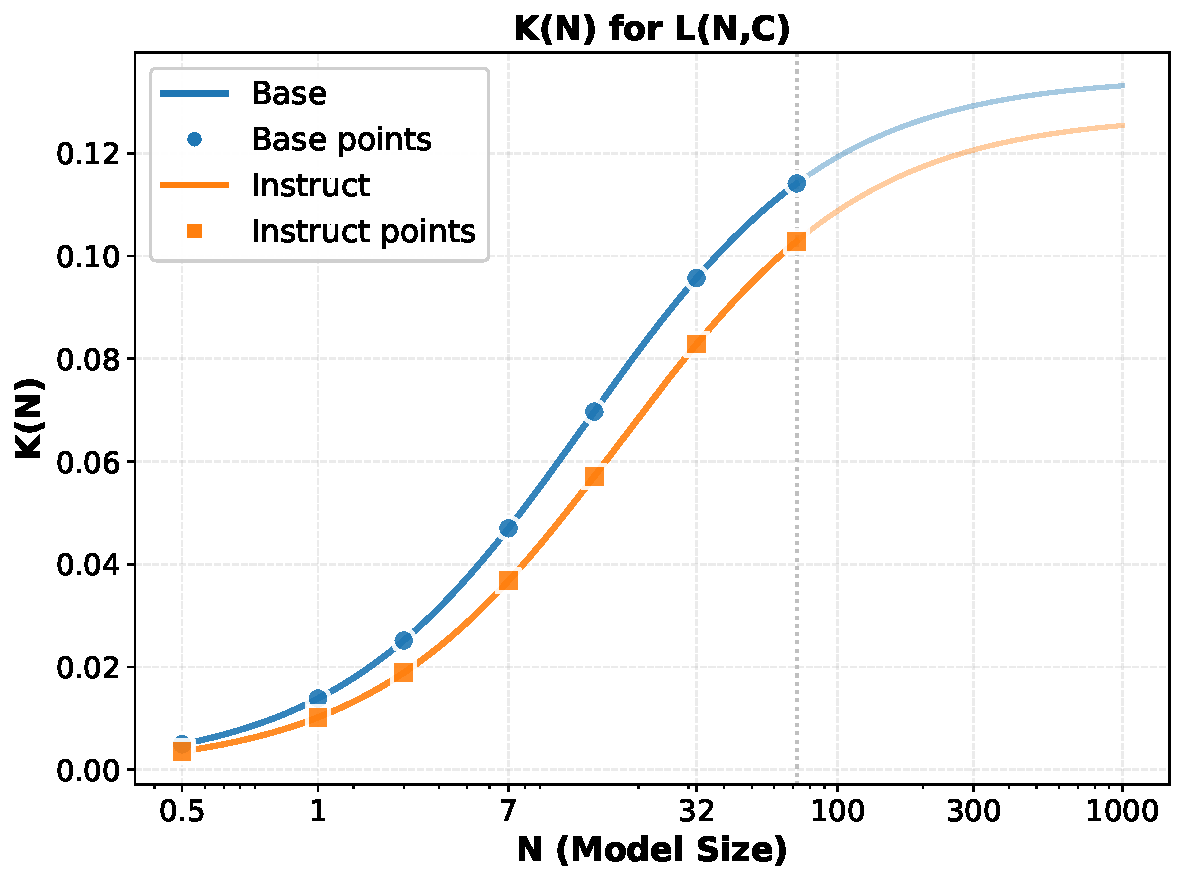
\includegraphics[width=\linewidth]{./figures/outputs/outputs/coefficient_k_intramodel_C.pdf}
        \caption{Fitted learning efficiency $k_C(N)$.} % 极简标题
        \label{fig:coef_k_c}
    \end{subfigure}
    \hfill % 左右留白
    % --- 右图 ---
    \begin{subfigure}[b]{0.49\textwidth}
        \centering
        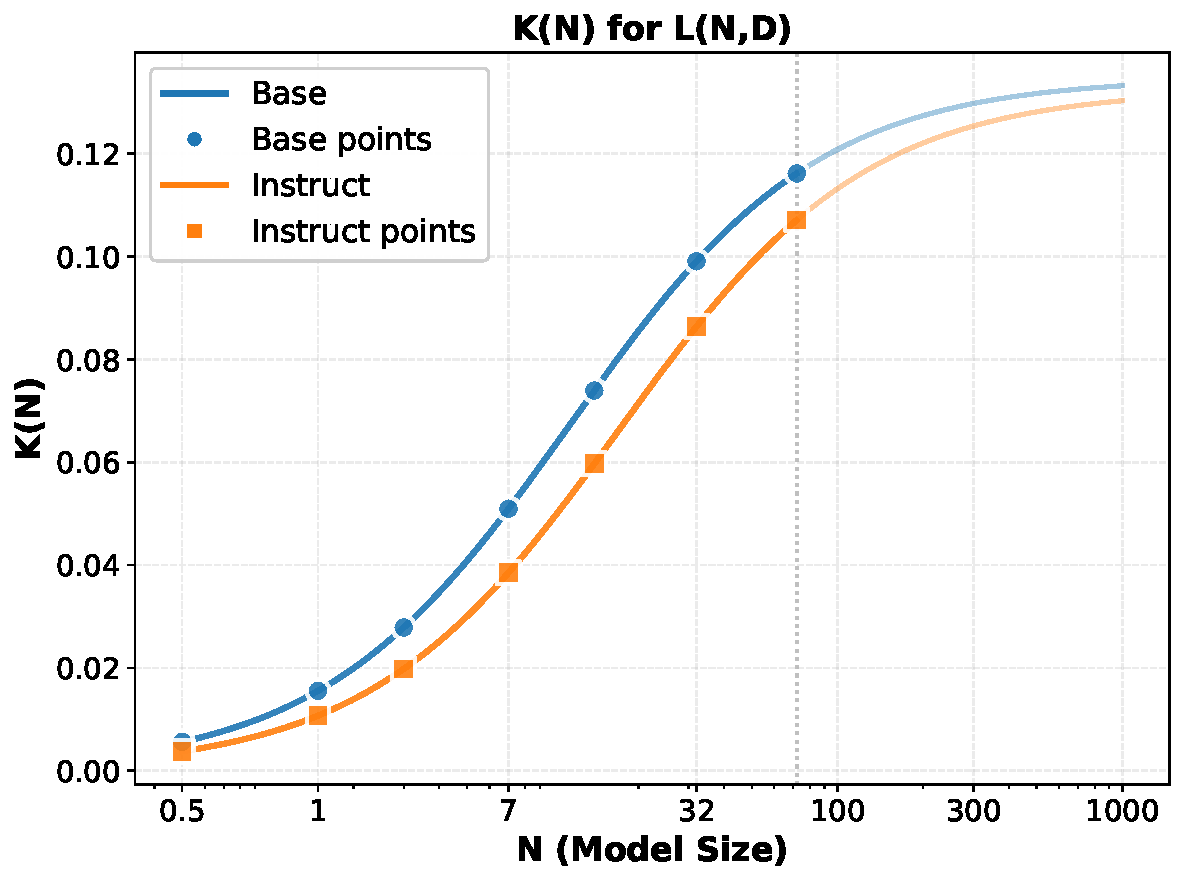
\includegraphics[width=\linewidth]{./figures/outputs/outputs/coefficient_k_intramodel_D.pdf}
        \caption{Fitted learning efficiency $k_D(N)$.} % 极简标题，长度一致
        \label{fig:coef_k_d}
    \end{subfigure}
    
    % --- 总标题 ---
    \caption{Fitted learning efficiency coefficients for Base and Instruct models. Both $k_C(N)$ (a) and $k_D(N)$ (b) exhibit identical trends: larger models consistently show higher learning efficiency, with efficiency gains beginning to diminish after the 32B model size.}
    \label{fig:coef_k_combined}
\end{figure*}




% \paragraph{\tzl{Unified Scaling Formulation and Predictive Power}} \tzl{Collectively, our analyses in Sections \ref{subsec:compute_scaling} and \ref{subsec:data_scaling} reveal that RL post-training follows a consistent power-law trajectory with respect to both compute and data. We identify a unified analytic form for the learning efficiency coefficient $k(N)$ (Eq. \ref{eq:compute_law} and Eq. \ref{eq:data_law}), which effectively captures the efficiency saturation observed as model size increases. More importantly, this formulation demonstrates robust predictive capabilities: as shown in Figures \ref{fig:loss_vs_compute_exp} and \ref{fig:loss_vs_data}, the empirical scaling law allows for accurate Inter-model Extrapolation (forecasting the performance of 72B models using parameters fitted on 0.5B-32B) and Intra-model Prediction (projecting the remainder of training from initial steps). These results demonstrate that the scaling dynamics of RL post-training in mathematical reasoning exhibit consistent and modelable patterns, providing a quantitative foundation for resource allocation.}
% \begin{figure}
%     \centering
%     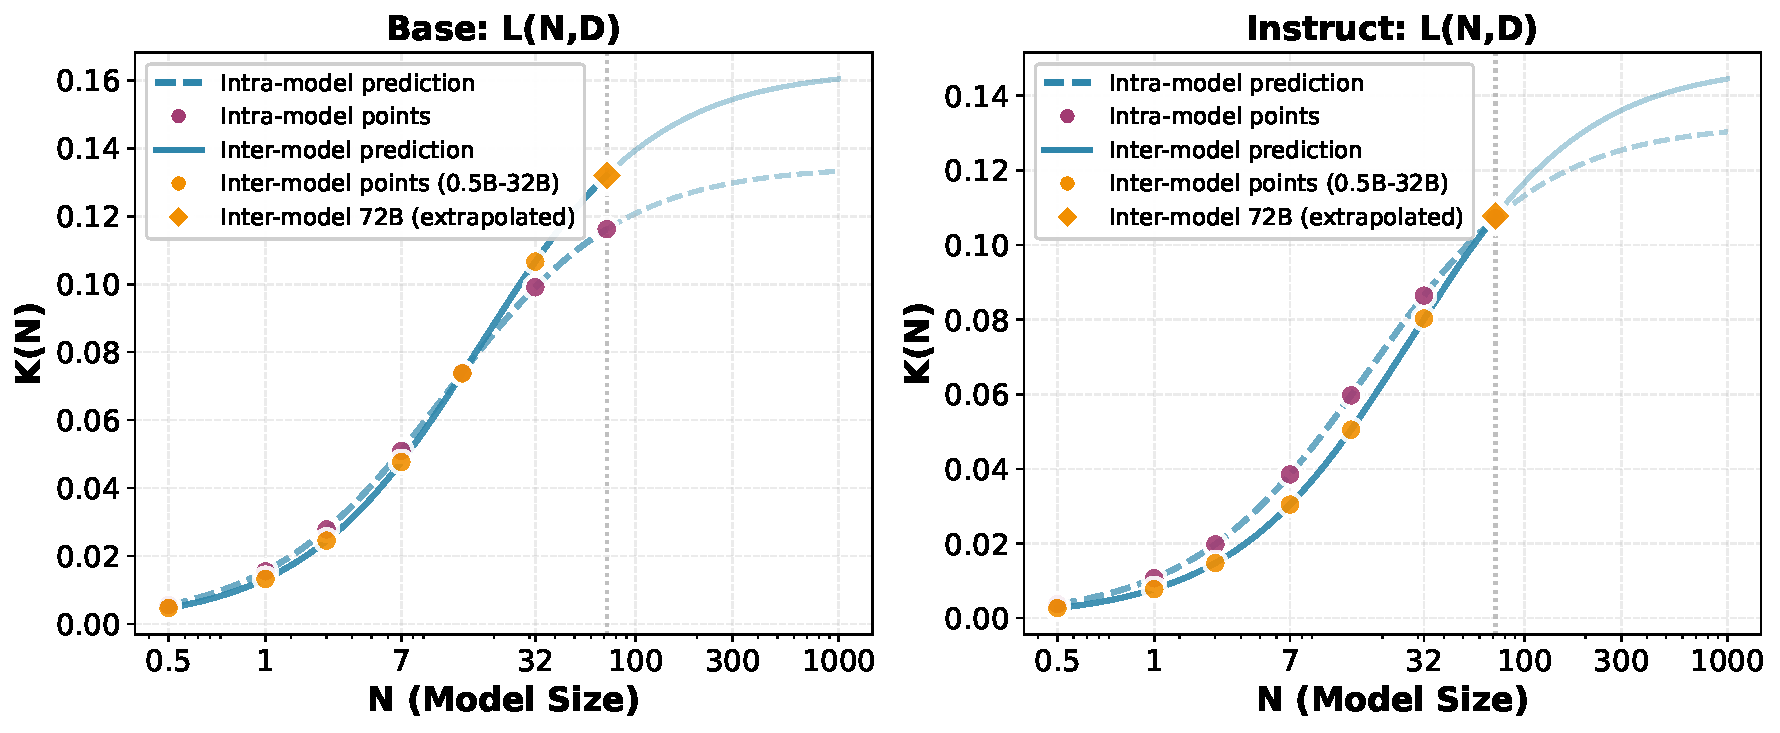
\includegraphics[width=0.7\linewidth]{.//figures//outputs//outputs/coefficient_k_predict_vs_extrap_D.pdf}
%     \caption{\tzl{Fitted learning efficiency coefficient $K(N)$ for the data scaling law $L(N,D)$ as a function of model size $N$ for Base and Instruct models}}
%     \label{fig:coef_k_d}
% \end{figure}
% \begin{table}[H]
% \centering
% \caption{Fitted slopes $k_D$ for different model sizes.}
% \label{tab:fitting_results_kd}
% \begin{tabular}{lccccc}
% \toprule
% \textbf{Model} & 0.5B & 1.5B & 3B & 7B & 14B \\
% \midrule
% Base     & 0.0070 & 0.0268 & 0.0181 & 0.0409 & 0.0739 \\
% Instruct & 0.0054 & 0.0065 & 0.0164 & 0.0469 & 0.0504 \\
% \bottomrule
% \end{tabular}
% \end{table}

% \begin{table}[H]
% \centering
% \caption{Fitted slopes $k_D$ for different model sizes.[TODO:Delete the table and let reader read infomation in Appendix]}
% \label{tab:fitting_results_kd}
% \resizebox{0.7\linewidth}{!}{%
% \begin{tabular}{lcccccccc}
% \toprule
% \textbf{Model} & 0.5B & 1.5B & 3B & 7B & 14B & 32B & 72B \\
% \midrule
% Base     & 0.0065 & 0.0247 & 0.0182 & 0.0450 & 0.0745 & 0.1072 & 0.1126 \\
% Instruct & 0.0052 & 0.0052 & 0.0155 & 0.0472 & 0.0502 & 0.0961 & 0.1094 \\
% \bottomrule
% \end{tabular}%
% }
% \end{table}

\subsection{Cross-Architecture Generalization}
\label{subsec:cross_arch}

\begin{figure*}[b]
    \centering
    \begin{subfigure}[b]{0.48\textwidth}
        \centering
        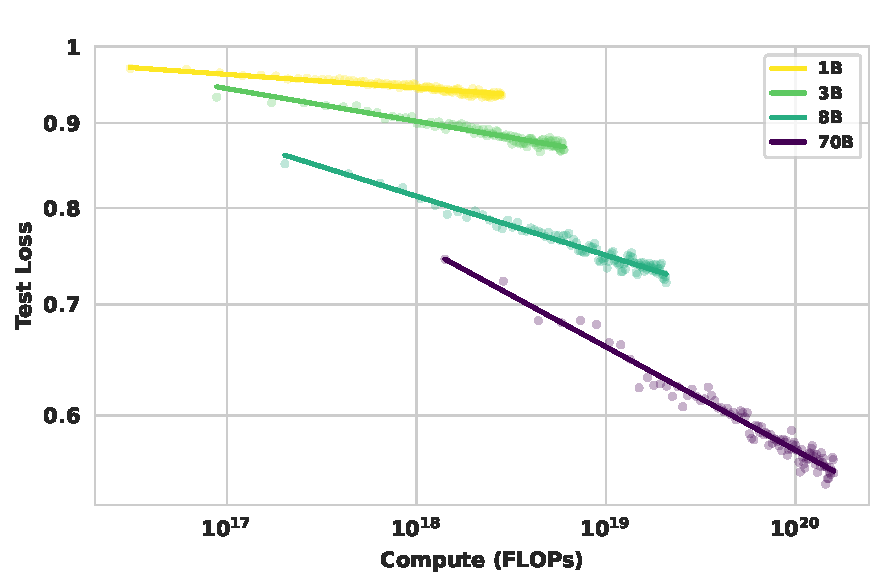
\includegraphics[width=\linewidth]{./figures/outputs/outputs/llama_paper_llama-instruct_holdout_N_C_raw_ErrRate.pdf}
        \caption{Fitted $L(N, C)$ on Llama Instruct}
        \label{fig:llama_scaling_c}
    \end{subfigure}
    \hfill
    \begin{subfigure}[b]{0.48\textwidth}
        \centering
        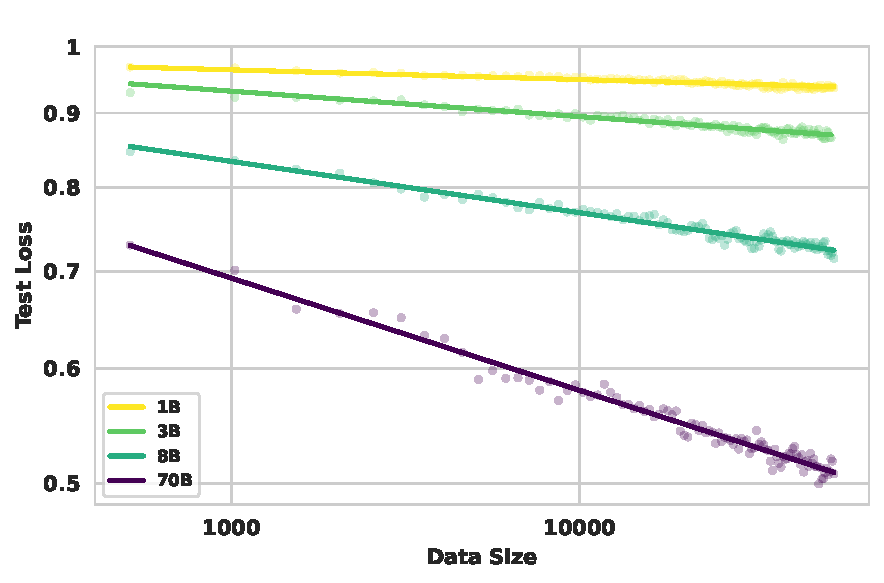
\includegraphics[width=\linewidth]{./figures/outputs/outputs/llama_paper_llama-instruct_holdout_N_E_ErrRate.pdf}
        \caption{Fitted $L(N, D)$ on Llama Instruct}
        \label{fig:llama_scaling_d}
    \end{subfigure}
    \caption{\textbf{Cross-architecture validation on Llama~3.} The same scaling law (Eq.~\ref{eq:compute_law},~\ref{eq:data_law}) fitted on Llama~3 Instruct models (1B--70B) achieves $R^2 > 0.99$ for both compute (a) and data (b) dimensions.}
    \label{fig:llama_scaling}
\end{figure*}

All experiments in Sections~\ref{subsec:compute_scaling} and~\ref{subsec:data_scaling} are conducted on the Qwen2.5 model family. A natural question is whether the observed scaling behavior is specific to a particular architecture or represents a more general property of RL post-training. To investigate this, we apply the same experimental protocol to the Llama~3 model family, spanning 1B to 70B parameters (Llama-3.2-1B/3B-Instruct and Llama-3.1-8B/70B-Instruct).

We train each model using identical GRPO configurations and evaluate on the same holdout benchmark. As shown in Figure~\ref{fig:llama_scaling}, both the compute scaling law $L(N,C)$ (Eq.~\ref{eq:compute_law}) and the data scaling law $L(N,D)$ (Eq.~\ref{eq:data_law}) fit the Llama results with $R^2 > 0.99$, confirming that the proposed log-linear formulation and the saturation structure of $k(N)$ generalize across architectures. Notably, while Llama models achieve lower absolute performance than Qwen at comparable sizes (e.g., Llama-70B peaks at ${\sim}50\%$ holdout accuracy vs.\ Qwen-72B at ${\sim}59\%$), the \emph{functional form} of the scaling relationship remains identical. This suggests that the scaling dynamics of RL post-training are governed by the optimization process itself, rather than by architecture-specific properties of the base model.


\subsection{Scaling with Constrained Data and Reuse}
When unique data is scarce, a critical question is whether repeating data is effective. We investigate this Data Reuse Scenario by fixing the total data budget and varying the reuse factor $\tau$. Specifically, we aim to identify the optimal reuse factor $\tau$ that minimizes the test loss:
\begin{equation}
\underset{\tau}{\text{argmin}} ; L(\tau) \quad \text{s.t.} \quad D_{\text{unique}} \times \tau = D_{\text{total}},\label{eq:data-reuse}
\end{equation}
\label{subsec:data_reuse}
To systematically evaluate this problem, we simulate data constraints by partitioning the training set into smaller subsets while preserving the difficulty distribution (Details provided in Appendix~\ref{app:data-reuse-detailed}). Each subset is cycled through multiple times, with $\tau$ controlling the repetition frequency. Crucially, the total number of used data $D_{\text{total}}$ is kept fixed across runs, and curriculum ordering is maintained to ensure that performance differences arise solely from the degree of data reuse rather than distributional artifacts.
\begin{figure}[H]
    \centering
    % --- Left Subfigure (Base model) ---
    \centering
    % Placeholder: Base model's Final Loss vs. Data Reuse Factor
    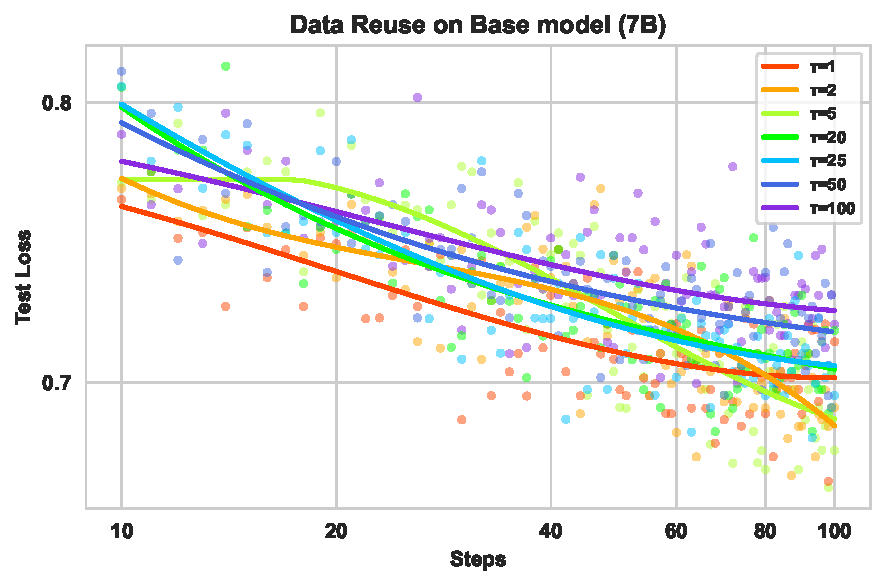
\includegraphics[width=\linewidth]{./figures/datareuse/fit_exp2-base_holdout_Tau_step_ErrRate.pdf}

    % --- Main Caption for the Entire Figure ---
    \caption{Performance in data-constrained settings is primarily determined by the total number of used data ($D_{\text{total}}$). For a fixed $D_{\text{total}}$, the final test loss is insensitive to the data reuse factor ($\tau$), with no significant degradation up to $\tau=25$.}
    \label{fig:data_reuse_ablation}
\end{figure}
Under this experimental setup, our results demonstrate that performance is primarily governed by the total number of optimization steps ($D_{\text{total}}$), rather than sample uniqueness. As illustrated in Figure~\ref{fig:data_reuse_ablation} (for instruct model, check Figure~\ref{fig:data_reuse_instruct} in Appendix~\ref{app:data-reuse-detailed}), the final test loss proves insensitive to the reuse factor, showing no significant degradation for $\tau \leq 25$. However, the limit exists at $\tau=100$, we observe clear signs of overfitting, indicating that excessive repetition eventually harms generalization. Collectively, these findings confirm that moderate data reuse is a highly effective strategy for RL fine-tuning in data-constrained regimes.


\subsection{Domain Transfer}
\label{subsec:domain-transfer}
\begin{figure*}[t]
    \centering
    % --- Left Subfigure (In-domain) ---
    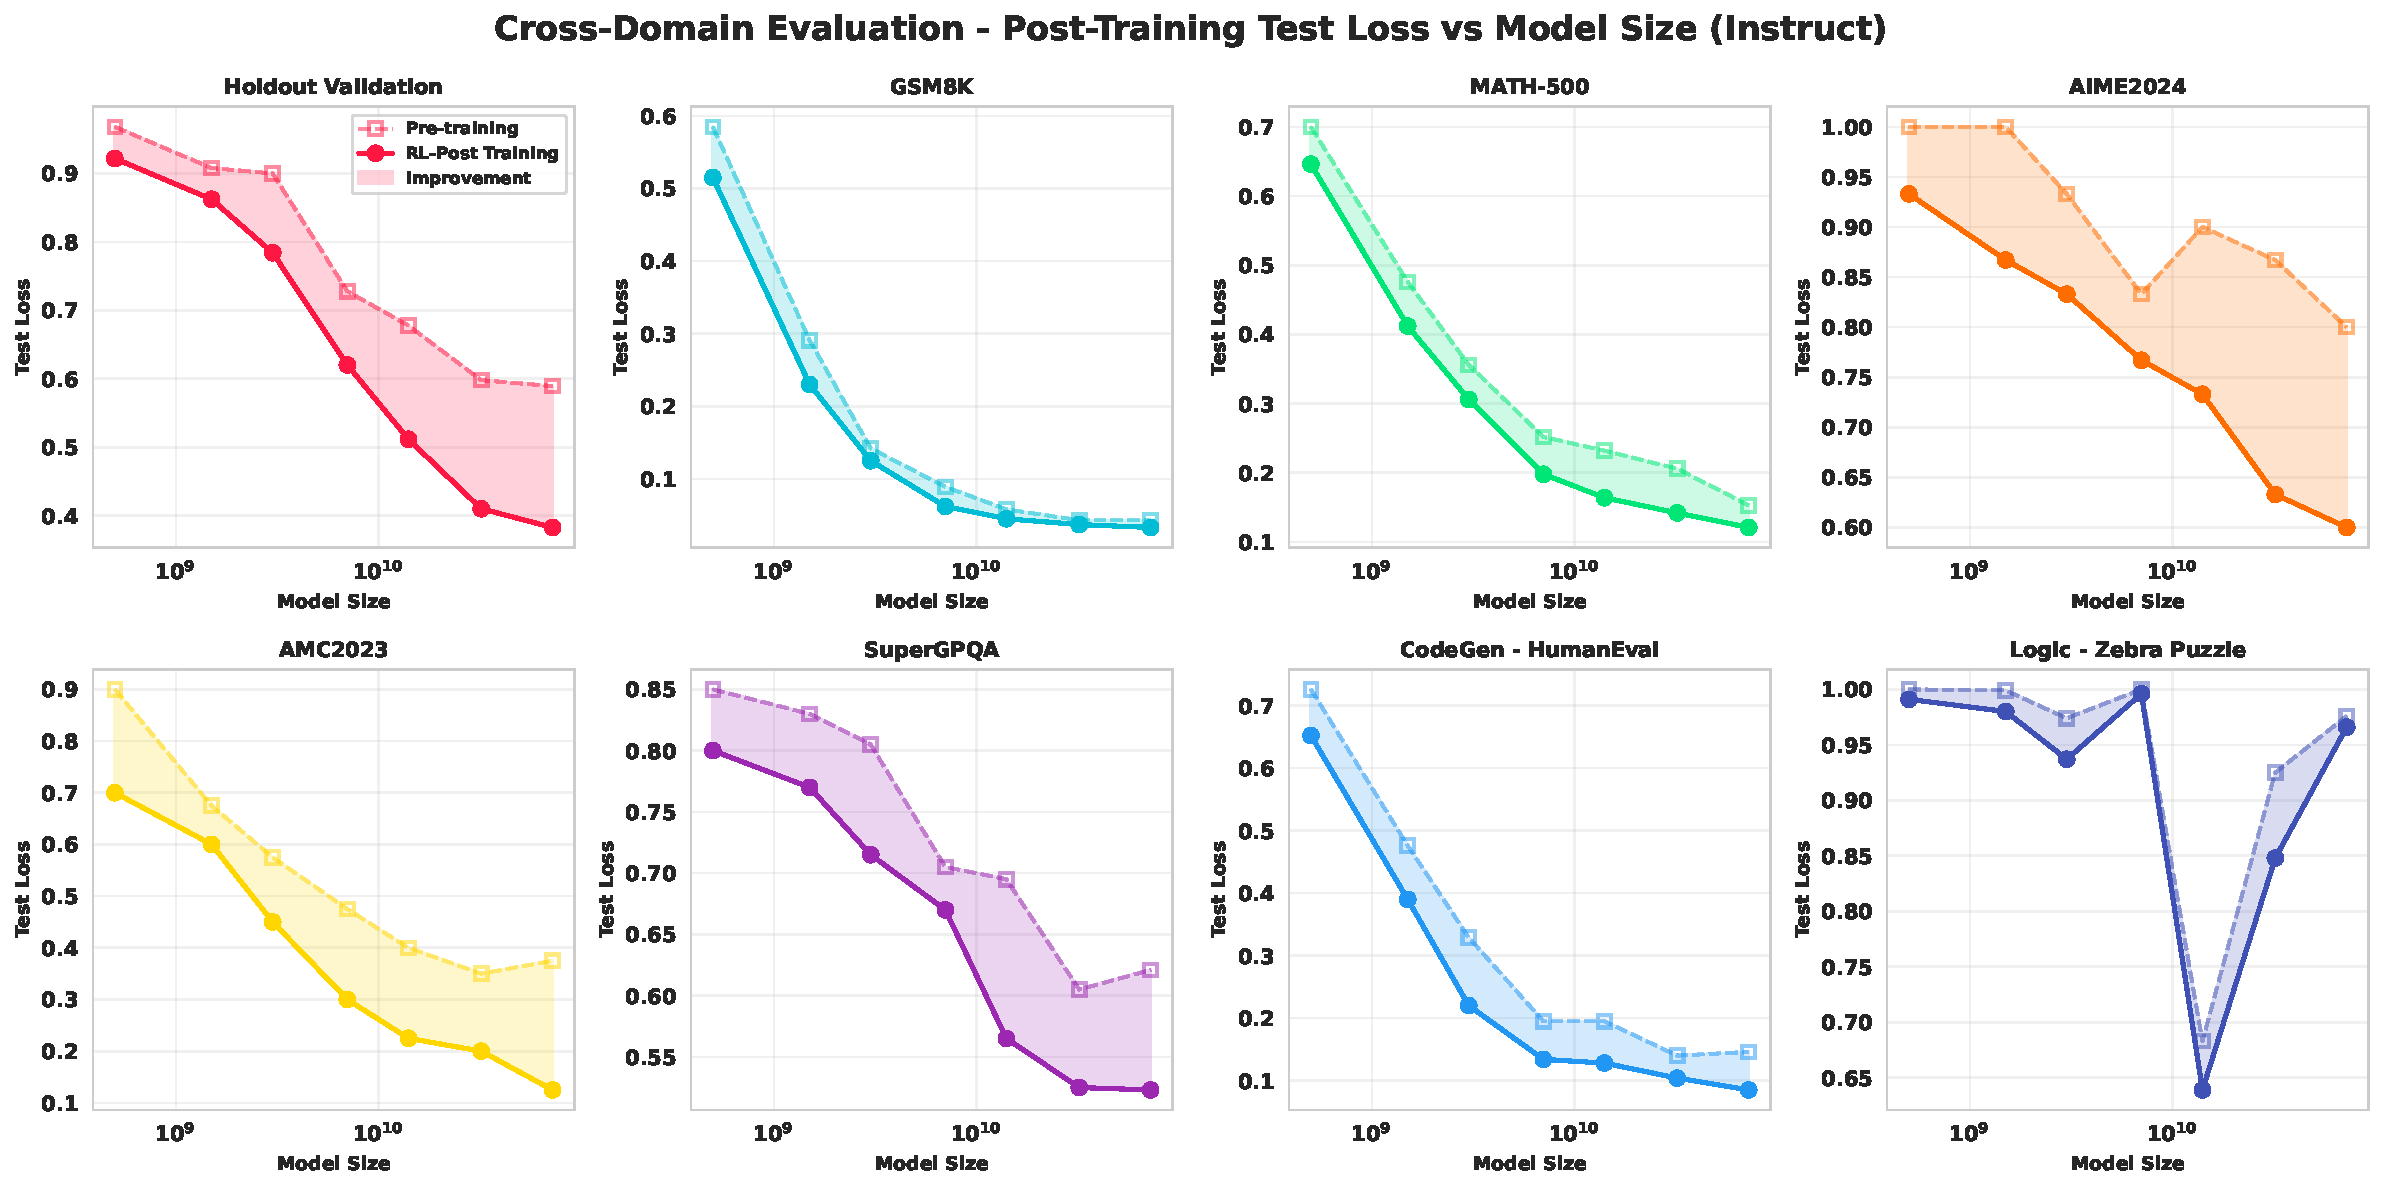
\includegraphics[width=\textwidth]{./figures/outputs/outputs/crossdomain_instruct_ErrRate_vs_N.pdf}
    \caption{\tzl{RL post-training on mathematical reasoning yields generalization improvements on in-domain tasks with varying difficulty, but shows negligible transfer to out-of-domain tasks.}}
    \label{fig:domain_transfer}
\end{figure*}
We investigate the generalization capabilities of reinforcement learning fine-tuning (RFT) by evaluating models on a comprehensive suite of in-domain and out-of-domain (OOD) benchmarks. Our results demonstrate a divergent trends: while RL post-training yields robust generalization improvements on in-domain mathematical tasks of varying difficulty, it shows negligible transfer to out-of-domain tasks. (Detailed results are provided in Appendix~\ref{app:generalization_tasks}).


\textbf{In-Domain Generalization.} Figure~\ref{fig:domain_transfer} shows consistent improvements on unseen mathematics tasks outside the training set. On benchmarks, from easy to hard, including \texttt{GSM8K}, \texttt{MATH-500}, \texttt{AMC2023}, \texttt{AIME2024}, test loss steadily decreases with training compute, suggesting that RL post-training enhances transferable reasoning skills within mathematics.


\textbf{Out-of-Domain Generalization.} As shown in Figure~\ref{fig:domain_transfer}, results on OOD tasks are markedly different. For code generation (\texttt{HumanEval}) and STEM problems (\texttt{SuperGPQA}), performance gains marginally, indicating that RL fine-tuning is highly specialized.\tzl{On logical reasoning (\texttt{zebra\_puzzle}), performance degrades for larger models, suggesting that intensive optimization on mathematical reasoning may interfere with or "damage" other distinct reasoning abilities}.


% \subsection{Ablation on GRPO Hyperparameters}
% \label{subsec:ablation_grpo}
% \begin{tcolorbox}[colback=blue!5!white, colframe=blue!30!white, title=Observation 6]
% A larger GRPO rollout group size ($G$) is consistently more data-efficient, while the compute-optimal $G$ grows with the total computational budget.
% \end{tcolorbox}
% \begin{figure}[h]
% \vskip -0.1in
%     \centering
%     \begin{subfigure}[t]{0.48\textwidth}
%         \centering
%         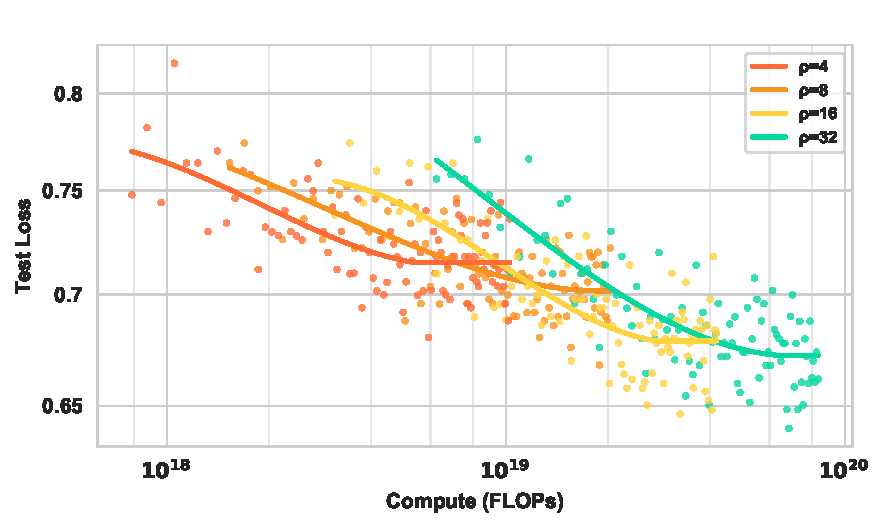
\includegraphics[width=\linewidth]{./figures/grpo/grpo_base_holdout_rollout_n_C_raw_ErrRate.pdf}
%         \caption{7B-Base: Loss vs.\ Compute}
%         \label{fig:grpo_ablation_a}
%     \end{subfigure}
%     \begin{subfigure}[t]{0.48\textwidth}
%         \centering
%         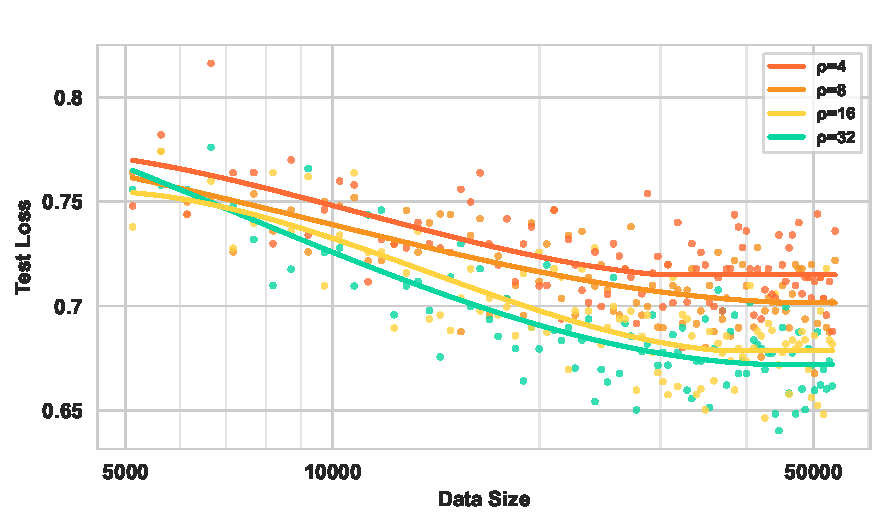
\includegraphics[width=\linewidth]{./figures/grpo/grpo_base_holdout_rollout_n_E_ErrRate.pdf}
%         \caption{7B-Base: Loss vs.\ Data Size}
%         \label{fig:grpo_ablation_b}
%     \end{subfigure}
    
%     \begin{subfigure}[t]{0.48\textwidth}
%         \centering
%         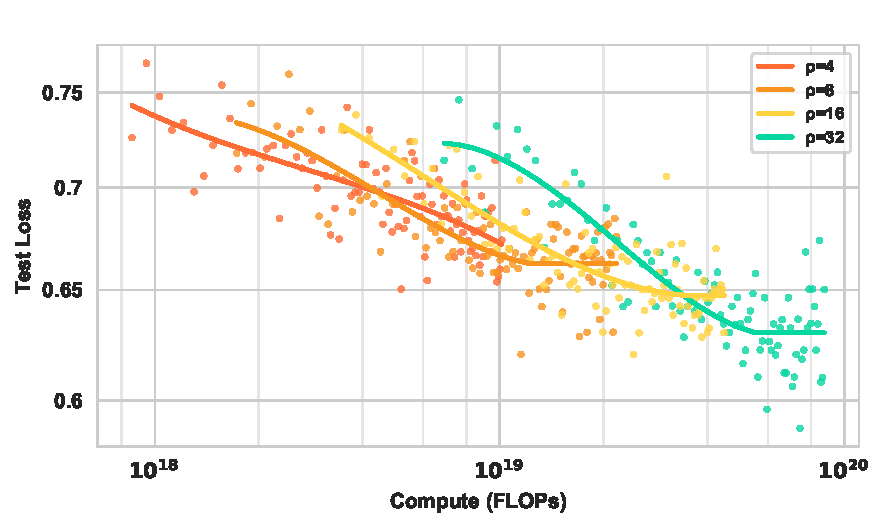
\includegraphics[width=\linewidth]{./figures/grpo/grpo_instruct_holdout_rollout_n_C_raw_ErrRate.pdf}
%         \caption{7B-Instruct: Loss vs.\ Compute}
%         \label{fig:grpo_ablation_c}
%     \end{subfigure}
%     \begin{subfigure}[t]{0.48\textwidth}
%         \centering
%         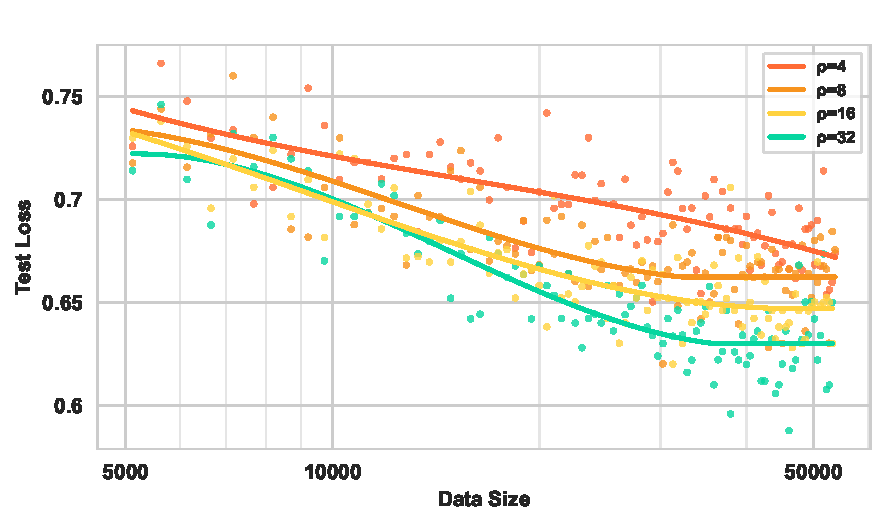
\includegraphics[width=\linewidth]{./figures/grpo/grpo_instruct_holdout_rollout_n_E_ErrRate.pdf}
%         \caption{7B-Instruct: Loss vs.\ Data Size}
%         \label{fig:grpo_ablation_d}
%     \end{subfigure}

%     \caption{
%         Effects of GRPO rollout size on training efficiency: (a–b) show compute/data scaling for 7B-Base; (c–d) for 7B-Instruct.
%     }
%     \label{fig:grpo_ablation}
%     \vskip -0.2in
% \end{figure}
% We conducted an ablation study on the rollout group size $G$, a key GRPO hyperparameter that controls how many responses are sampled per prompt. This directly affects both the compute per update and the stability of the training signal. We tested $G \in \{4, 8, 16, 32\}$ on the 7B models.

% \textbf{Data-centric View}. Figure~\ref{fig:grpo_ablation_b} and \ref{fig:grpo_ablation_d} shows that larger rollout sizes consistently yield better sample efficiency: $G=32$ achieves the lowest test loss for the same number of unique samples. This supports the intuition that more responses per question provide a stronger advantage estimate and thus more effective gradient updates.

% \textbf{Compute-centric View}. The optimal rollout size $G$ is not fixed but shifts with the training budget. 
% This implies that practitioners should tune $G$ according to available compute rather than relying on a universal setting. 
% We attribute this dynamic to the trade-off between the higher variance reduction from larger $G$ and the additional FLOPs it consumes, which makes small $G$ preferable at low budgets but large $G$ superior when ample compute is available.




